Das Polynom $m(X)=X^2+X+1$ ist als Polynom in $\mathbb{F}_3[X]$ irreduzibel.
Dies bedeutet, dass der Ring der Polynome $\mathbb{F}_3[X] / (m(X))$ 
ein Körper ist, man bezeichnet ihn auch mit $\mathbb{F}_3(\alpha)$,
wobei man sich $\alpha$ als eine Nullstelle von $m(X)$
oder als die Matrix
\[
\alpha = \begin{pmatrix} 0&2\\1&2\end{pmatrix}
\]
vorstellen kann.
\begin{teilaufgaben}
\item 
Stellen Sie die Additions- und Multiplikationstabellen für das Rechnen
in $\mathbb{F}_3$ auf.
\item
Berechnen Sie $\alpha^{-1}$ in $\mathbb{F}_3(\alpha)$ aus der
Bedingung $m(\alpha)=0$.
\item
Verwenden Sie den euklidischen Algorithmus, um $(1+\alpha)^{-1}$
in $\mathbb{F}_3(\alpha)$ zu bestimmen.
\item
Berechnen Sie $\alpha^3$.
\end{teilaufgaben}

\begin{loesung}
\begin{teilaufgaben}
\item
Die Additions- und Multiplikationstabelle von $\mathbb{F}_3$ ist
\begin{center}
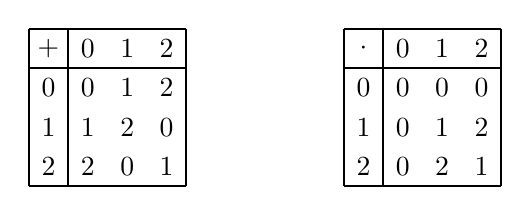
\begin{tikzpicture}[>=latex,thick]
\def\ds{0.5}
\def\punkt#1#2{({(#1)*\ds},{-(#2)*\ds})}
\def\tabelle{
\foreach \x in {-0.5,0.5,3.5}{
	\draw \punkt{\x}{-0.5} -- \punkt{\x}{3.5};
	\draw \punkt{-0.5}{\x} -- \punkt{3.5}{\x};
}
\node at \punkt{0}{1} {$0$};
\node at \punkt{0}{2} {$1$};
\node at \punkt{0}{3} {$2$};
\node at \punkt{1}{0} {$0$};
\node at \punkt{2}{0} {$1$};
\node at \punkt{3}{0} {$2$};
}
\begin{scope}[xshift=-2cm]
\tabelle
\node at \punkt{0}{0} {$+$};
\node at \punkt{1}{1} {$0$};
\node at \punkt{1}{2} {$1$};
\node at \punkt{1}{3} {$2$};
\node at \punkt{2}{1} {$1$};
\node at \punkt{2}{2} {$2$};
\node at \punkt{2}{3} {$0$};
\node at \punkt{3}{1} {$2$};
\node at \punkt{3}{2} {$0$};
\node at \punkt{3}{3} {$1$};
\end{scope}
\begin{scope}[xshift=2cm]
\tabelle
\node at \punkt{0}{0} {$\cdot$};
\node at \punkt{1}{1} {$0$};
\node at \punkt{1}{2} {$0$};
\node at \punkt{1}{3} {$0$};
\node at \punkt{2}{1} {$0$};
\node at \punkt{2}{2} {$1$};
\node at \punkt{2}{3} {$2$};
\node at \punkt{3}{1} {$0$};
\node at \punkt{3}{2} {$2$};
\node at \punkt{3}{3} {$1$};
\end{scope}
\end{tikzpicture}
\end{center}
\item
Wegen $m(\alpha)=\alpha^2+\alpha+1=0$ folgt $\alpha+1+\alpha^{-1}=0$
oder $\alpha^{-1} = -\alpha - 1 = 2+2\alpha$.
Als Matrix kann man
\[
\alpha^{-1}
=
2\alpha + 2
=
\begin{pmatrix}
0&4\\
2&4
\end{pmatrix}
+
\begin{pmatrix}
2&0\\0&2
\end{pmatrix}
=
\begin{pmatrix}
2&4\\2&2
\end{pmatrix}
\equiv
\begin{pmatrix}2&1\\2&0\end{pmatrix}
\mod 3
\]
schreiben und durch Nachrechnen verifizieren dass, tatsächlich gilt
\[
\alpha\alpha^{-1}
=
\begin{pmatrix}
0&2\\
1&2
\end{pmatrix}
\begin{pmatrix}
2&1\\
2&0
\end{pmatrix}
=
\begin{pmatrix}
4&0\\
6&1
\end{pmatrix}
\equiv
\begin{pmatrix}
1&0\\
0&1
\end{pmatrix}
\mod 3.
\]
\item
Für den euklidischen Algorithmus müssen wir wiederholt eine Polynomdivision
in $\mathbb{F}_3[X]$ durchführen.
Im ersten Schritt ist es
\[
\arraycolsep=1.4pt
\begin{array}{rcrcrcrcrcr}
 \llap{$($}X^2&+&X&+&1\rlap{$)$}&\;:&(X&+&1)&=&X = q_1\\
\llap{$-($}X^2&+&X\rlap{$)$}& &  & &  & &  & & \\ \cline{1-3}
     & &0&+&1 &\rlap{$\mathstrut = r_1$}\phantom{)}& &  & &  & \\
\end{array}
\]
Die nächste Division ist $(X+1) : 1$, die als Quotient $q_2=X+1$ und den
Rest $r_2=0$ hat.
Mit der Matrixform des euklidischen Algorithmus kann man jetzt auch die
Koeffizienten $s$ und $t$ bestimmen, die beide Polynome in $\mathbb{F}_3[X]$
sind:
\begin{align*}
Q
&=
Q(q_2)
Q(q_1)
=
\begin{pmatrix}
0&1\\1&-q_2
\end{pmatrix}
\begin{pmatrix}
0&1\\1&-q_1
\end{pmatrix}
=
\begin{pmatrix}
0&1\\1&2X+2
\end{pmatrix}
\begin{pmatrix}
0&1\\{\color{red}1}&{\color{red}2X}
\end{pmatrix}
=
\begin{pmatrix}
{\color{red}1}&{\color{red}2X}\\
2X&X^2+X+1
\end{pmatrix}.
\end{align*}
Die gesuchten Polynome sind $s=1$ und $t=2X$ und man kann nachrechnen,
dass
\begin{align*}
s\cdot m(X) + t\cdot (X+1)
&=
X^2+X+1 + 2X\cdot (X+1)
=
X^2+X+1 + 2X^2 + 2X
\\
&= 3X^2+3X+1\equiv 1 \mod 3.
\end{align*}
Natürlich kann man $s$ und $t$ auch mit der erweiterten Tabelle
finden:
\begin{center}
\begin{tabular}{|>{$}c<{$}|>{$}c<{$}>{$}c<{$}|>{$}c<{$}|>{$}c<{$}|>{$}c<{$}>{$}c<{$}|}
\hline
k&    a_k&b_k& q_k&r_k& c_k&     d_k\\
\hline
 &       &   &    &   &   1&       0\\
0&X^2+X+1&X+1& X  &  1&   0&       1\\
1&    X+1&  1& X+1&  0&{\color{red}   1}&{\color{red}      2X}\\
2&      1&  0&    &  0&2X+2& 2X^2+2X\\
\hline
\end{tabular}
\end{center}
In allen Fällen ist also $(1+X)^{-1} = 2X$.
\item
Wegen $m(\alpha)=0$ ist $\alpha^2=-\alpha-1=2\alpha+2$ und damit
\begin{align*}
\alpha^3
&=
\alpha\cdot \alpha^2 = \alpha (2\alpha +2) = 
2\alpha^2 + 2\alpha
=
2(\underbrace{\alpha^2 + \alpha + 1}_{\displaystyle=0} + 2)
=
2\cdot 2
=
1.
\qedhere
\end{align*}
\end{teilaufgaben}
\end{loesung}
